\documentclass[12pt]{article}
\usepackage{amsmath} % for the equation* environment
\usepackage{graphicx} % for inserting images
\graphicspath{{./plots/}} % plots directory
\usepackage{float} % to fix position of figures
\usepackage[a4paper, margin=1.5cm]{geometry} % paper size and margins
\usepackage[skip=10pt, indent=0pt]{parskip} % paragraph sep and identation
\usepackage{caption} % to change figure caption size
\captionsetup[figure]{font=footnotesize,labelfont=bf}
\usepackage{xcolor}
\definecolor{bg}{gray}{0.97}
\usepackage{minted} % for code blocks
\setminted{
    linenos=True,
    %bgcolor=bg,
    frame=single,
    framesep=2.5mm,
    baselinestretch=1.2,
}
\usepackage[hidelinks]{hyperref} % for links

\setcounter{tocdepth}{2} % Only show sections and subsections in the TOC

\title{High-level programming paradigm comparison}
\author{Iyán Méndez Veiga \and Jingzhi Zhang}
\date{HPC4WC SS-2023}

\begin{document}

\maketitle
\tableofcontents

\section{Introduction}

Python~\cite{Python} is great for quickly developing and validating new ideas and algorithms. It is also an excellent language for sharing code with others since its simple syntax---quite close to mathematical-style pseudocode---makes the code very readable. However, Python is also noticeably slower when compared to other languages used in high-performance computing, such as Fortran, C/C++, or Rust. There are several reasons for this, which will be briefly explained in this introduction. The goal of this project is to explore a few different high-level programming techniques to accelerate Python code and to conduct a performance and usability analysis.

Many factors can cause a program to run slowly. Even a high-performance computing program written in C can take a long time to execute if it spends a significant amount of time waiting. This can happen, for example, when there are I/O tasks such as reading or writing files from disk. However, in this project, we will not be concerned about this type of \emph{slowness}. Our focus is on CPU tasks: understanding why Python executes CPU tasks more slowly than other languages and attempting to reduce this performance gap using high-level programming accelerators.

\subsection{Why is Python slow?}

\paragraph{Python is dynamically typed} This means that when writing Python code, we do not have to worry about the types of the variables. We can even reuse the same variable with different types in different parts of the code. This is not possible in C or Fortran, both of which are examples of statically typed languages.

\paragraph{Python is an interpreted language} Before running any program written in a compiled language, such as C or Fortran, the source code has to be converted into machine code. This machine code consists of the exact instructions that the CPU needs to execute when running the program. Python, on the other hand, operates differently. The source code is translated into platform-independent bytecode, which does not include direct instructions for the CPU but rather something that the Python interpreter can understand. Subsequently, this bytecode is further translated into CPU instructions by the Python interpreter.

And all this happens at runtime! Python's slower performance stems from the fact that, unlike statically typed and compiled languages, the compilation and interpretation of the code happen when we execute the program, not before when we compile the source code.

\paragraph{Python is single-threaded on a single CPU} Furthermore, contrary to other languages, Python is single-threaded on a single CPU by design. This is enforced by the Global Interpreter Lock (GIL), which ensures that the Python interpreter only executes one thread at a time. The reason for enforcing this by design is due to how Python manages memory. Not only do we not have to worry about specifying the type of variables, but we also do not have to take care of allocating the right amount of memory and freeing it when we are done with that variable. All of this is handled for us by the Python interpreter, but it comes at a (performance) cost.

\subsection{High-level programming accelerators}

Performance of pure python code can be improved by carefully using the built-in C modules (e.g., the function \texttt{range()}), and some of the packages from the standard library to bypass, for example, the GIL when possible (e.g., \texttt{asyncio}, \texttt{threading} and \texttt{multiprocessing}). This, however, is something out of the scope of this project.

\subsubsection{NumPy}

For scientific calculations, replacing tuples or lists with NumPy~\cite{NumPy} arrays, and the math functions from the standard library \texttt{math} with the vectorized NumPy ones is a great way to speed up the code. The gain in performance comes from the fact that the core of NumPy is well-optimized C code. Since NumPy relies on an accelerated linear algebra library, compiling NumPy against a faster algebra library can lead to further performance gains. This is the case, for example, when compiling NumPy with Intel MKL instead of OpenBLAS on Intel CPUs. For this project, though, we have used the standard NumPy wheels available on PyPI, which are built against OpenBLAS.

\subsubsection{Numba}

What if we could easily compile certain parts of our Python code to benefit from the performance of compiled languages while retaining the simplicity and readability of the original Python code? This is exactly what Numba~\cite{Numba} aims for, by translating Python functions to optimized machine code at runtime. Because everything happens at runtime, there is no need to replace the Python interpreter or run an additional compilation step before running the Python code. Numba does everything for us. On top of that, Numba also provides some tools to simplify writing stencil computations.

\subsubsection{GT4Py}

As we have learnt during the course~\cite{HPC4WC}, GT4Py~\cite{GT4Py} is a Domain Specific Language (DSL) designed for weather and climate modeling on Python. It is mainly based on the C++ library GridTools which provides automatic optimizations according to the CPU and GPU information, and it still maintains Python's readability. By compiling stencils in GT4Py style one can benefit from low-level acceleration, multi-core paralleling and GPU acceleration.

\subsubsection{NumExpr}

NumExpr~\cite{NumExpr} is an accelerator for computations involving element-wise operations on NumPy arrays. It achieves better performance than NumPy by avoiding intermediary arrays in memory and taking advantage of multi-threaded computations using all available cores. By design, it is not straightforward to accelerate general stencil computations with NumExpr although, as we will show later, there is way around this using array views.

\subsubsection{Taichi}

Taichi~\cite{Taichi} is also a DSL designed to optimize visual computing and physics simulation algorithms with its imperative programming paradigm. With also the Just-In-Time (JIT) compiling and parallel threading over CPUs or GPUs, Taichi can help accelerate stencil computations. It is specially designed for optimizing graphic visualization, machine learning and spatially sparse data processing, which, however, will not be involved in our case.

\subsection{Stencil computations}

As we have learned in the course, a stencil computation on a grid is an algorithm that updates the value of each gridpoint following exactly the same pattern and using only other gridpoints from a compact neighborhood. For the purposes of this project we have selected five difference stencils to update 3D fields:

\begin{enumerate}
    \item Pointwise copy
    \begin{equation*}
        a[i,j,k] = b[i,j,k]
    \end{equation*}
    \item Pointwise sine
    \begin{equation*}
        a[i,j,k] = \sin(b[i,j,k])
    \end{equation*}
    \item 1D same column update
    \begin{equation*}
        a[i,j,k] = \frac{1}{2}\Big(b[i+1,j,k] - b[i,j,k]\Big)
    \end{equation*}
    \item 1D same row update
    \begin{equation*}
        a[i,j,k] = \frac{1}{2}\Big(b[i,j+1,k] - b[i,j,k]\Big)
    \end{equation*}
    \item Diffusion operator
    \begin{equation*}
        \frac{\partial\phi}{\partial t} = -\alpha \Delta(\Delta\phi))
    \end{equation*}
    The explicit stencil is obtained by doing a 2nd-order centered spatial discretization and a 1st-order forward time discretization.
    \begin{align*}
    a_n[i,j,k] &= \Delta(\Delta b_n[i,j,k])) \\
    &= 20\, b_n[i,j,k] - 8 \Big(b_n[i+1,j,k] + b_n[i-1,j,k] + b_n[i,j+1,k] + b_n[i,j-1,k]\Big)\\
    &\quad + 2\Big(b_n[i+1,j+1,k] + b_n[i+1,j-1,k] + b_n[i-1,j+1,k] b_n[i-1,j-1,k]\Big) \\
    &\quad + b_n[i+2,j,k] + b_n[i-2,j,k] + b_n[i,j+2,k] + b_n[i,j-2,k]\\
    a_{n+1}[i,j,k] &= a_n[i,j,k] - \alpha\, b_n[i,j,k]
    \end{align*}
\end{enumerate}

The first stencil is a simple copy without any computation, which will allow us to better understand how different Python objects are stored in memory, determine the Python overhead of running nested loops, and study how good different high-level accelerators are at overcoming this. The second stencil includes a small computation which will be helpful to benchmark the performance of different accelerators. The third and forth stencils will allow us to determine the impact of data storage in memory and how we access it to maximize cache hit ratio. Lastly, the diffusion operator is the same we have used during the course and it is an example of a stencil computation that is used in current weather and climate simulations. This will allow us to benchmark the accelerators with a realistic stencil computation.

\subsection{Structure of the project repository}

Our project is in \texttt{<HPC4WC repo>/projects/2023/project12\_highlevel\_programming} and it consists of:
\begin{itemize}
    \item a setup script: \texttt{setup.sh}, which should be run once to create the Python virtual environment and the Jupyter kenel in the CSCS JupyterHub,
    \item listed dependencies: \texttt{requirements.txt} for \texttt{pip}, \texttt{pyproject.toml} for package management, and \texttt{pdm.lock} for \texttt{pdm},
    \item a \texttt{Makefile} to generate this report from its source \texttt{report.tex},
    \item a small Python module, \texttt{common.py}, containing some useful functions,
    \item six self-contained Jupyter Notebooks where all our tests are explained in detail,
    \item and a \texttt{results.csv} file containing all the benchmark results after running the notebooks in the CSCS Jupyter Hub.
\end{itemize}

\section{Benchmark \& Usability analysis}

The goal of this project is to determine how much performance gain we can obtain using a few high-level programming accelerators. Equally important, we want to learn how easy it is to use these accelerators and how readable the new code is. As the base case to compare we will use spatial loop-free NumPy code taking advantage of vectorized mathematical functions. But before doing that we decided to explore exactly how fast NumPy really is compared to pure Python code or, in other words, how large the overhead of looping and indexing is in these stencil computations, as well as trying to better understand how Python lists and NumPy arrays are stored in memory.

For all the tests we have used 3D fields with dimensions $(\text{NX}, \text{NY}, \text{NZ}) = (128,128,80)$ iterating the stencil computations 50 times. Fields are initialized with different patterns to validate the correctness of our implementations, but benchmarks are always run with randomly initialized fields, with a seeded PRNG for reproducibility.

\subsection{Lists vs NumPy arrays}

In this section we summarize the main results from the Jupyter notebook \href{run:./1_lists_numpy.ipynb}{\texttt{1\_lists\_numpy.ipynb}}.

\subsubsection{Python lists}

The CPython implementation of Python lists can be found in a header in the CPython GitHub repository~\cite{CPython}. Essentially, Python lists are vectors of pointers. Each list element is a pointer to a valid Python object (of any type). 3D fields, therefore, can be constructed as nested lists. For example, we can create a list with \texttt{NZ} lists, where each of these lists is also a list with \texttt{NY} further more lists, and where, finally, each of these lists is a list with \texttt{NX} floats. In this way, accessing the field element $\phi(x,y,z)$ is done by reading the element \texttt{field[z][y][x]}.

Because of how Python lists are implemented, they are very flexible objects. They can be enlarged, reduced, and new elements can be inserted or deleted at arbitrary positions. This comes at a cost: Python lists are not cache friendly. This partly explains why working with large 3D fields as lists is very slow. But even if CPU cache utilization is not ideal, we can still notice some effect in performance depending on how we iterate the lists. Results can be observed in the Jupyter notebook where we tried the 6 possible permutations for the order of the \texttt{for} loops. The main takeaway is that nested Python lists should be looped in the same order they are nested.

\subsubsection{NumPy arrays}

NumPy arrays are not exactly what one would expect when hearing the word array, specially for C or Fortran developers. NumPy arrays can be split into two parts: the data buffer (what C/Fortran people would expect to be an array) and the metadata about the data buffer. The data buffer is a contiguous and fixed block of memory containing fixed-sized data items. And the metadata about the data buffer contains a lot of extra information to interpret correctly the data buffer such as the basic data element's size in bytes, the number of dimensions, the separation between elements for each dimension (i.e., the strides), the byte order of the data, the data type which allows the correct interpretation of the basic data elements in Python, and whether the data buffer is row-major (C-style) or col-major (Fortran-style).

NumPy will always try, when possible, to do changes to the metadata part without changing the data buffer. For example, when we swap the order of dimensions, or select a part of an array (slicing), or transpose it, all these changes do not modify the data buffer. Using NumPy terminology, these are different views of the same underlying data buffer. This is great when working with NumPy because most of the times we will not loose performance by making unnecessary copies of data, but it also makes it more difficult to optimize the code and one has to be careful when working with high-level accelerators. Most of the surprising or unexpected results we found while working on this project could always be explained keeping in mind the internal organization of NumPy arrays.

\subsubsection{Results}

NumPy is a great high-level accelerator for scientific calculations, and in particular it achieves a great performance gain with stencil computations when compared to Python lists due to higher cache hit ratios. This only happens when arrays are used with vectorized code though, which, unfortunately, can worsen code readability in some situations. NumPy code of the pointwise sine stencil is 16 times faster than pure Python code, and the 1D stencil is 150 times faster.

Interestingly, using the simplest of the five stencils (copy) and NumPy arrays of different sizes, we were able to determine the size of the L3 cache (details in the last Appendix of the Jupyter notebook).


\subsection{Numba}

Numba is explored in detail in the Jupyter notebook \href{run:./2_numba.ipynb}{\texttt{2\_numba.ipynb}}. Numba is a large, widely used and well documented project. We selected a few of the most relevant features to test against our stencil computations. In particular, we tested the decorator \texttt{@numba.jit()} to compile our Python functions into machine code, the decorator \texttt{@numba.stencil()} to define the stencil computation using relative coordinates, and the replacement \texttt{numba.prange()} to parallelize the loop over the Z dimension, in a similar way to using OpenMP with C or Fortran.

The Numba code of the pointwise sine stencil is 220 times faster than pure Python code, and 14 times faster than the vectorized NumPy code. For the 1D stencils, it is 30 times faster than the vectorized NumPy code, for the 2D stencil it is 65 times faster. Our benchmarks are in agreement with the claims in the official documentation, where they mention that speedups can go from one to two orders of magnitude.

In terms of usability, Numba is great. The only problem is that vectorized NumPy code needs to be rewritten using \texttt{for} loops to iterate over the arrays. Once we have such code, we obtain a huge boost in performance by just adding a single line of code on top of our Python functions. For people not familiar with NumPy slicing and vectorized expressions, Numba code is even more readable.

\subsection{GT4Py}

GT4Py is explored in detail in the Jupyter notebook \href{run:./3_gt4py.ipynb}{\texttt{3\_gt4py.ipynb}}. We tested several backends available for GT4Py and supported on CSCS, including \texttt{numpy} which is ``a vectorized Python backend'', \texttt{gt:cpu\_ifirst} ``targeting many core architectures'' and \texttt{gt:cpu\_kfirst} ``performance-optimized for x86 architecture'', to see their performance for stencil processing. By introducing the decorator \texttt{@gtscript.stencil(backend=...)} or the function \texttt{gtscript.stencil(backend=..., definition=definition\_function)}, we can compile a GT4Py stencil with a certain backend. The data is managed in the form of \texttt{gt.storage} class, so that the data backend would be consistent with the stencil backend setting.

Although the GT4Py code of the pointwise stencil is slower than the vectorized NumPy code, it is about 15 times faster when operating on the 1D stencil with \texttt{backend="gt:cpu\_kfirst"} and 33 times faster on the 2D stencil with \texttt{backend="gt:cpu\_ifirst"}. For the 2D stencil, GT4Py is able to optimize the slowest part of the diffusion calculation reducing the computation time from about 20 ms, in the case of NumPy, to about 600 $\mu$s.

The usability of GT4Py is not as good as Numba. Even though the \texttt{@gtscript.stencil} decorator helps users to code in a easier way, you have to define the data type of all variables in the stencil, and also the external functions. Other than that, data have to be converted into \texttt{gt.storage} type. To get the most out of GT4Py, users should also know how an array is read from memory, so that they can choose the best origin index that an array is most frequently read, as well as which backend would perform best for a specific task.

\subsection{NumExpr}

NumExpr is introduced and tested in the Jupyter notebook \href{run:./4_numexpr.ipynb}{\texttt{4\_numexpr.ipynb}}. NumExpr is a much more specialized accelerator than Numba. Similar to GT4Py, it aims to accelerate a very particular task, in this case element-wise mathematical operations in very large NumPy arrays. It is actively maintained, although documentation could be improved.

Unfortunately, our stencil computations did not benefit much from NumExpr. The reason is that all our stencils have very simple mathematical operations. In addition, by design, NumExpr cannot deal with general stencil computations (other than pointwise ones). We showed how to overcome this limitation by using array views for the 1D stencil.

In conclusion, NumExpr can be an interesting accelerator to optimize performance and memory usage when dealing with large element-wise operations. The performance gained against vectorized NumPy code should be tested also against a Numba accelerated version, so that the best option for each particular scenario is chosen. In terms of usability, NumExpr is extremely easy to use, although everything is done through its main routine \texttt{numexpr.evaluate()} rather than wrapping some already existing functions in a decorator, or replacing \texttt{numpy} with \texttt{numexpr} at import time.


\subsection{Taichi}

Taichi is introduced and tested in the Jupyter notebook \href{run:./5_taichi.ipynb}{\texttt{5\_taichi.ipynb}}. Taichi compiles the functions using the \texttt{@ti.kernel} or \texttt{@ti.func} decorators. The data can be either NumPy arrays or its own data structure called \texttt{field}. Aside from the automatic JIT compiling, GPU and parallel acceleration can also be implemented depending on the settings. It is a very popular solution for visual computing and physics simulation, and it can also accelerate deep learning code.

Taichi codes generally perform well on CSCS for our testings thanks to its support to GPU acceleration, similar to other DSLs in most other tasks after specific optimization. In the task of pointwise sine calculation, Taichi reached the highest speed with CUDA backend, about 56 times faster than the NumPy approach. For the 1D stencils, it is only 5.2 times faster than the NumPy code, for the 2D stencil it is 46 times faster. As Taichi is more designed for heavy computation, we expect to see better performances when using larger arrays.

However, adapting source code to Taichi is very tricky. For example, the compiling unit in Taichi, called \texttt{kernel}, forbids the usual data swap codes, so we had to use the much slower ``\texttt{copy\_from}" workaround. Besides, kernels cannot return multi-dimension arrays, and treat arrays as global variables, but prohibits its change after compiling for the first time. Very careful coding is needed to fully exploit Taichi. The advantage of Taichi is that we can simply switch or restart the kernel by one command, thus enabling simple optimization using different backends.


\section{Results \& Conclusion}

During this project we have studied and understood in detail how Python lists and NumPy arrays are stored in memory. This allowed us to explain some, \emph{a priori}, surprising results in terms of optimal cache utilization. We have also explored and tested in detail a few different high-level accelerators. The following plots summarize our results for the different accelerators.

\begin{figure}[H]
    \centering
    \includegraphics[width=0.8\textwidth]{pointwise_copy_stencil.eps}
    \caption{In this plot we can see the different run times (log scale) for the copy stencil. Unsurprisingly, the slowest implementations are the pure Python one using nested lists and the one using NumPy arrays but keeping the for loops. These two implementations are in the order of tens of seconds. The fastest implementation is the vectorized NumPy one, which is around 5 orders of magnitude faster that the slowests. However, this huge boost in performance, as explained in the Appendix of \href{run:./1_lists_numpy.ipynb}{\texttt{1\_lists\_numpy.ipynb}}, cannot be reproduced for larger arrays once they stop fitting into L3 cache. All the accelerators tested managed to reduce the run time to the order of ms or tens of ms.}
    \label{fig:stencil_copy}
\end{figure}

\begin{figure}[H]
    \centering
    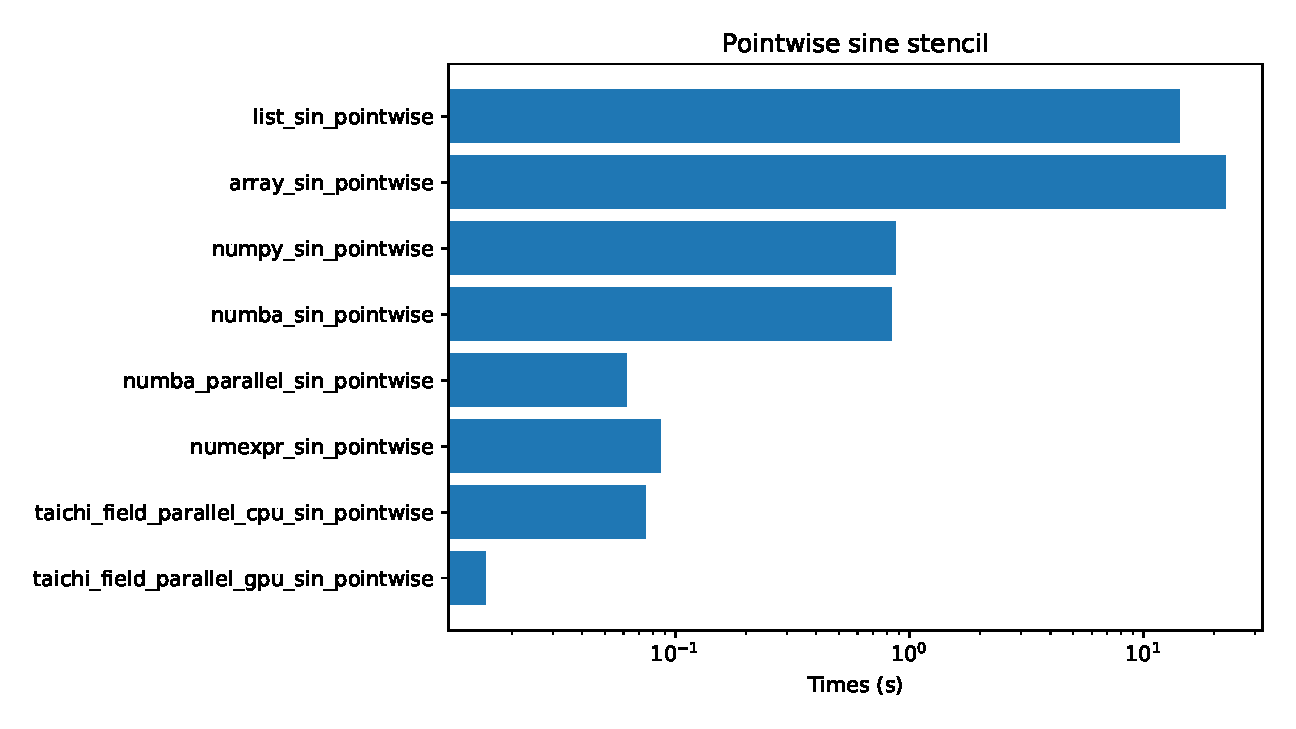
\includegraphics[width=0.8\textwidth]{pointwise_sine_stencil.eps}
    \caption{In this plot we show the run times (log scale) of the pointwise sine stencil. Similarly to the copy stencil results, the pure Python and array with loops are the slowest implementations. The Numba single-threaded accelerated implementation is almost identical to the vectorized NumPy one, which gives us confidence in the statement that the core of NumPy is well-optimized C code. However, Numba can also generate machine code that uses all the available cores, improving the run time one further order of magnitude. In this case, the fastest implementation is the Taichi using the GPU backend.}
    \label{fig:stencil_sine}
\end{figure}

\begin{figure}[H]
    \centering
    \includegraphics[width=0.8\textwidth]{1d_stencil.eps}
    \caption{In this plot we show the run times (log scale) of one of the 1D stencils we considered in the project. The array with loops version was not implemented since it was already clear from the pointwise stencils that it was slower than the pure Python implementation. Almost all accelerated implementations improve the performance from the tens of seconds obtained with the nested lists to hundreds of ms. GT4Py using the optimized backend for x86 and Numba achieve further performance gain, reducing the run time to just a few ms.}
    \label{fig:stencil_1D}
\end{figure}

\begin{figure}[H]
    \centering
    \includegraphics[width=0.8\textwidth]{2d_stencil.eps}
    \caption{In this plot we show the run times (log scale) of the 2D stencil implementing the diffusion operator used during the course. All accelerators managed to improve the reference implementation using vectorized NumPy code, except GT4Py with the NumPy backend. Numba, Taichi and GT4Py (with ifirst and kfirst backends) achieve similar speedups with run times in the order of tens of ms.}
    \label{fig:stencil_2D}
\end{figure}

More detailed explanations can be found on our Jupyter notebooks. We conclude that Numba is the best option to accelerate stencil computations both in terms of performance and usability, at least for the considered stencils and in the single node scenario. However, many of the accelerators explored in this project are under rapid and active development, so it might be interesting to revisit these benchmarks in the future. There are other accelerators that might be interesting to accelerate stencil computations and have not been tested in this project. For example, JAX~\cite{Jax}, currently being developed by Google, can accelerate NumPy and pure Python code by compiling to GPUs and even TPUs. Although focused on machine learning, perhaps stencil computations are also a good fit, and it could be interesting for a future project.

\newpage
\begin{thebibliography}{9}
    \bibitem{Python} The Python Tutorial — Python 3.11.5 documentation.\\\href{https://docs.python.org/3/tutorial/index.html}{https://docs.python.org/3/tutorial/index.html}

    \bibitem{NumPy} NumPy documentation — NumPy v1.25 Manual.\\\href{https://numpy.org/doc/stable}{\texttt{https://numpy.org/doc/stable}}

    \bibitem{Numba} Numba documentation — Numba 0.57.1.\\\href{https://numba.readthedocs.io/en/stable/index.html}{\texttt{https://numba.readthedocs.io/en/stable/index.html}}
    
    \bibitem{HPC4WC} GitHub Repository: HPC4WC: High Performance Computing for Weather and Climate.\\\href{https://github.com/ofuhrer/HPC4WC}{\texttt{https://github.com/ofuhrer/HPC4WC}}

    \bibitem{GT4Py} GT4Py: GridTools for Python — GT4Py 1.0.0 documentation.\\ \href{https://gridtools.github.io/gt4py/latest/index.html}{\texttt{https://gridtools.github.io/gt4py/latest/index.html}}
    
    \bibitem{NumExpr} NumExpr Documentation Reference.\\\href{https://numexpr.readthedocs.io/en/latest/index.html}{\texttt{https://numexpr.readthedocs.io/en/latest/index.html}}

    \bibitem{Taichi} Taichi Docs.\\\href{https://docs.taichi-lang.org}{\texttt{https://docs.taichi-lang.org}}

    \bibitem{CPython} GitHub Repository: CPython, \texttt{listobject.h}\\\href{https://github.com/python/cpython/blob/main/Include/cpython/listobject.h}{\texttt{https://github.com/python/cpython/blob/main/Include/cpython/listobject.h}}

    \bibitem{Jax} JAX: High-Performance Array Computing — JAX documentation.\\\href{https://jax.readthedocs.io/en/latest}{\texttt{https://jax.readthedocs.io/en/latest}}
\end{thebibliography}

\end{document}
